\documentclass[a4paper,12pt]{article}

% don't forget the document class, generally : \documentclass[a4paper,12pt]{article}

\usepackage[utf8]{inputenc}
\usepackage[french]{babel}
\usepackage{graphicx}
\usepackage{gensymb}
\usepackage{amsmath}
\usepackage{float}
\usepackage{scrextend}
\usepackage{caption} 
\usepackage{siunitx}
\usepackage{enumitem}
\usepackage{amsthm}
\usepackage{fancyhdr}
\usepackage{amssymb}
\usepackage{wrapfig}
\usepackage{geometry}
\usepackage{standalone}
\usepackage{import}
\usepackage[usenames, dvipsnames]{color}

 \usepackage{biblatex} % manages bibliography and references
\addbibresource{sample.bib}


\geometry{hmargin=1in, vmargin=1in}

 \newenvironment{absolutelynopagebreak}
 {\par\nobreak\vfil\penalty0\vfilneg
 \vtop\bgroup}
 {\par\xdef\tpd{\the\prevdepth}\egroup
 \prevdepth=\tpd}
 
 \pagestyle{fancy}                        
\fancyhf{}                               
\fancyhf[HL]{Application des maths}                
\fancyhf[HR]{Géométrie euclidienne}             
\fancyhf[FC]{\thepage/\pageref{Lastpage}}
 
\newtheorem{definition}{Définition}[section]
\newtheorem{theorem}{Théorème}
\newtheorem{corollary}{Corollaire}[theorem]
\newtheorem{lemma}[theorem]{Lemme}
\newtheorem*{hyp}{Hypothèse}
\newtheorem*{concl}{Conclusion}
\newtheorem*{remark}{Remarque}

\captionsetup{format=default,labelformat=simple,labelsep=colon,
justification=justified,font={sf,small},labelfont=bf,
textfont=default} 



\begin{document}

\pagebreak
\begin{corollary}
Deux triangles qui ont respectivement un côté et deux angles isométriques sont isométriques.
\end{corollary}

\begin{proof}
Considérons deux triangles $\triangle a_1b_1c_1$ et $\triangle a_2b_2c_2$.

\begin{figure}[H]
    \centering
    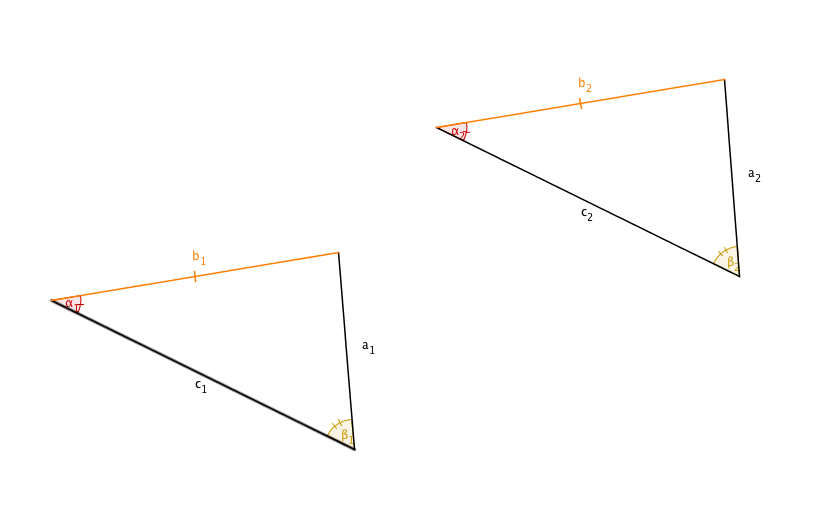
\includegraphics[scale=0.5]{schema/Corrolaire.png}
\end{figure}

\begin{hyp}
$a \equiv a'$, $\beta \equiv \beta'$ et $\alpha \equiv \alpha'$
\end{hyp}
\begin{concl}
$b \equiv b'$, $c \equiv c'$ et  $\gamma \equiv \gamma'$
\end{concl}

Pour démontrer ce corollaire, nous avons superposé ces deux triangles. Il existe alors trois cas possibles:
\begin{enumerate}
    \item $c_1 \equiv c_2$
    \item $c_1 > c_2$
    \item $c_1 < c_2$
\end{enumerate}
Dans le premier cas, comme $c_1 \equiv c_2$, $\beta_1 \equiv \beta_2$ et $a_1 \equiv a_2$, on sait que les deux triangles sont isométriques (axiome III).\\
Dans les deux autres cas, on peut observer la formation du triangle $b_1b_2'c_3$, dont l'un des angles est alpha 1. Considérons ce triangle, on peut observer que l'un de ses angles externes (voir sous-section 6.1) est $\alpha_2$, ce qui implique que $\alpha_1 < \alpha_2$, ce qui est absurde. Le seul cas possible est donc le premier.
\begin{figure}[H]
    \centering
    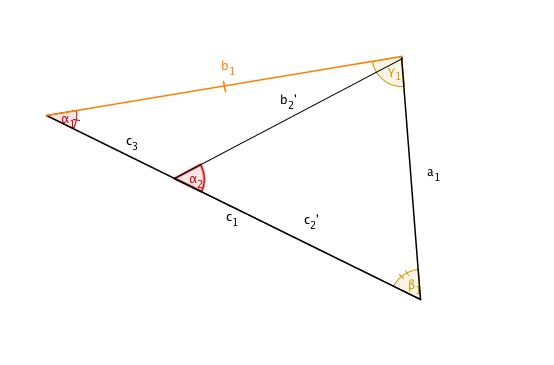
\includegraphics[scale=0.6]{schema/Corrolaire2.png}
\end{figure}
\end{proof}

\begin{remark}
Un corollaire est une démonstration nouvelle que l'on peut faire grâce à une affirmation précédente. Le mot provient du latin "corollarium", qui signifie littéralement "petite couronne".\footnote{CNRTL, dictionnaire étymologique, http://www.cnrtl.fr/}
\end{remark}

\end{document}